\documentclass[10pt]{article}
\usepackage[utf8]{inputenc}
\usepackage[spanish]{babel}
\usepackage{amsmath}
\usepackage{amsfonts}
\usepackage{amssymb}
\usepackage{graphics}
\usepackage{graphicx}
\usepackage[left=2cm,right=2cm,top=2cm,bottom=2cm]{geometry}
\usepackage{imakeidx}
\makeindex[columns=3, title=Alphabetical Index, intoc]
\usepackage{listings}
\usepackage{xcolor}
\usepackage{multicol}
\usepackage{changepage}
\usepackage{float}
\usepackage{cite}
\usepackage{url}
\usepackage{hyperref}
\usepackage{pdflscape}
\usepackage[document]{ragged2e}
\hypersetup{
    colorlinks=true,
    linkcolor=blue,
    filecolor=magenta,
    urlcolor=blue,
}

\definecolor{codegreen}{rgb}{0,0.6,0}
\definecolor{codegray}{rgb}{0.5,0.5,0.5}
\definecolor{codepurple}{rgb}{0.58,0,0.82}
\definecolor{backcolour}{rgb}{0.95,0.95,0.92}

\lstdefinestyle{mystyle}{
    backgroundcolor=\color{backcolour},
    commentstyle=\color{codegreen},
    keywordstyle=\color{magenta},
    numberstyle=\tiny\color{codegray},
    stringstyle=\color{codepurple},
    basicstyle=\ttfamily\footnotesize,
    breakatwhitespace=false,
    breaklines=true,
    captionpos=b,
    keepspaces=true,
    numbers=left,
    numbersep=5pt,
    showspaces=false,
    showstringspaces=false,
    showtabs=false,
    tabsize=3
}
\def\fillandplacepagenumber{%
 \par\pagestyle{empty}%
 \vbox to 0pt{\vss}\vfill
 \vbox to 0pt{\baselineskip0pt
   \hbox to\linewidth{\hss}%
   \baselineskip\footskip
   \hbox to\linewidth{%
     \hfil\thepage\hfil}\vss}}
\lstset{style=mystyle}

\title{Centro de Investigación en Cómputo\\Instituto Politécnico Nacional\\Metaheurísticas\\Actividad Cuestionario Examen Tema I\\Curso impartido por: Dra Yenny Villuendas Rey}

\author{Adrian González Pardo}

\date{\today}

\newcommand\tab[1][1cm]{\hspace*{#1}}

\begin{document}
\maketitle
\section{Preguntas}
\begin{center}
  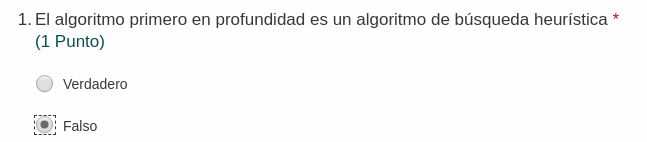
\includegraphics[scale=0.5]{img/p1.png}
\end{center}
\textit{Justificación 1: }No es un algoritmo heurístico ya que el algoritmo heurístico busca partir de una solución y de forma aleatoria ir mejorándolo, mientras que la búsqueda por profundidad e incluso por anchura se realiza de forma ordenada, partiendo de un nodo origen y ya sea con backtracking o con fuerza bruta busca encontrar la solución.\\
\begin{center}
  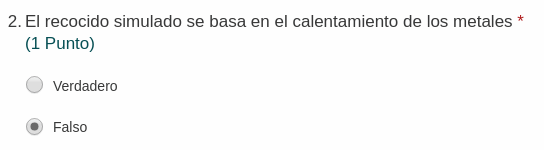
\includegraphics[scale=0.5]{img/p2.png}
\end{center}
\textit{Justificación 2: }El algoritmo si es referente a calentar metales, pero a su vez también se trata acerca del enfriamiento del mismo, entonces al ser una respuesta parcial referente a lo que es el Recocido Simulado no se puede tomar como respuesta valida.\\


\begin{center}
  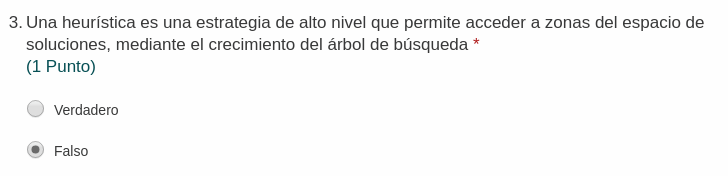
\includegraphics[scale=0.5]{img/p3.png}
\end{center}
\textit{Justificación 3: }Las heurísticas si funcionan como un árbol pero el crecimiento del árbol funciona cortando los nodos aledaños formando una ruta de exploración por lo cual siento que esta incompleta esta respuesta.\\


\begin{center}
  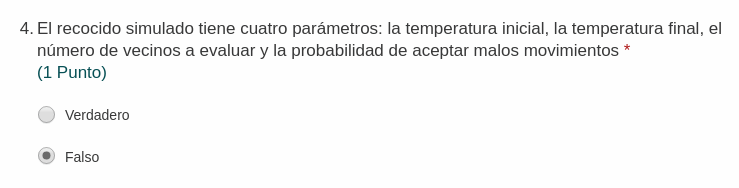
\includegraphics[scale=0.5]{img/p4.png}
\end{center}
\textit{Justificación 4: }Si bien estos 4 elementos son los participes del algoritmo SA, no son todos los parámetros ya que falta el parámetro $\alpha$ el cual nos ayuda a bajar la temperatura y quizás hacer la indicación del parámetro delta el cual nos dice explícitamente si se trata de optimizar con minimización o con maximización.\\

\begin{center}
  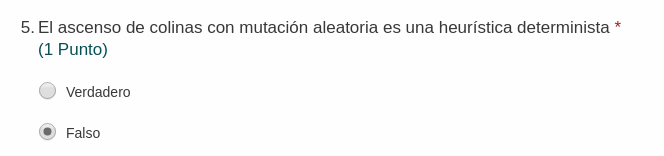
\includegraphics[scale=0.5]{img/p5.png}
\end{center}
\textit{Justificación 5: } Esto es debido a que inicialmente buscamos una solución aleatoria la cual va a ser modificada de forma aleatoria bajo una cadena de bits el cual representara casillas a intercambiar o en su defecto un índice a modificar, por ello no puede ser determinista, ya que no sigue un patrón exacto de pasar de un estado a otro.\\

\begin{center}
  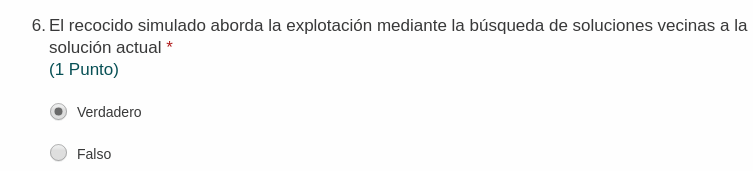
\includegraphics[scale=0.5]{img/p6.png}
\end{center}
\textit{Justificación 6: }Es verdadero ya que al obtener inicialmente una solución aleatoria comenzamos a modificar a partir de ella y de las sutiles modificaciones, obtenemos un vecino el cual sera evaluado en una función costo, contra la primer solución y de acuerdo a si se busca minimizar o maximizar este sera aceptado como nueva solución o en su defecto pasara por la función de probabilidad el cual nos dirá si se acepta el error de solución para así escapar del "mínimo local" (en ocasiones puede ser el mínimo global).\\

\begin{center}
  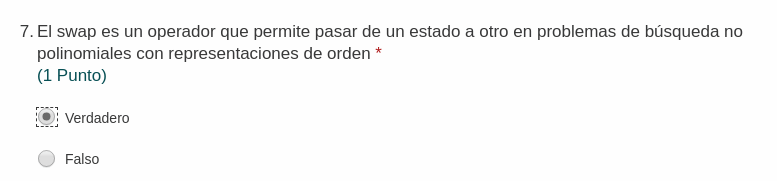
\includegraphics[scale=0.5]{img/p7.png}
\end{center}
\textit{Justificación 7: }Es verdadero ya que el operador de swap dependiendo del problema y de la heurística nos permite modificar la solución inicial y pasar a una nueva solución la cual puede ser mejor o en su defecto, puede que no lo sea.\\

\begin{center}
  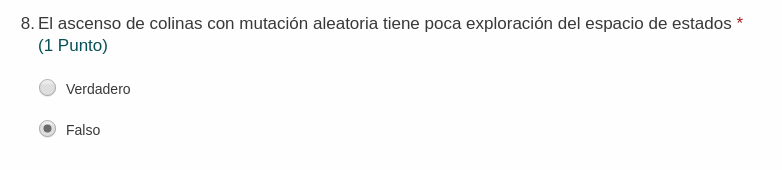
\includegraphics[scale=0.5]{img/p8.png}
  % Esta estuvo mal
\end{center}
\textit{Justificación 8: }Es falso ya que depende mucho de como se comience a explorar o de donde parta nuestra solución aleatoria, como bien puede partir de una solución peor evaluada, e ir modificándose a mejor solución sobre cada iteración, como bien puede que no.\\

\begin{center}
  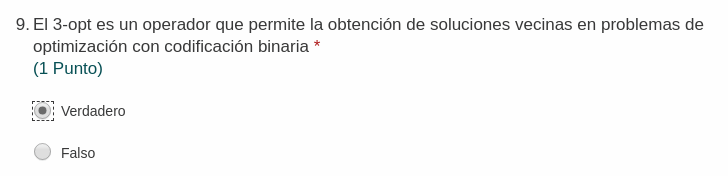
\includegraphics[scale=0.5]{img/p9.png}
  % Esta estuvo mal
\end{center}
\textit{Justificación 9: }Esta respuesta depende mucho respecto a la implementación de la solución al TSP, pero igual puede que si la solución parte de un vector entero, puede que esta respuesta pase como el caso contrario, es decir, sea falsa.\\

\begin{center}
  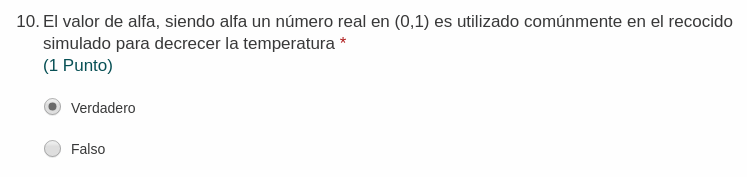
\includegraphics[scale=0.5]{img/p10.png}
\end{center}
\textit{Justificación 10: }Si bien es verdadero lo que hace el parámetro $\alpha$ también depende de como se determine el dominio de selección del valor aleatorio ya que en algunos papers seleccionan un $\alpha\in[0.88,0.99]$.

\end{document}
